\newenvironment{myitemize} % hacks
{ \begin{itemize}
    \setlength{\itemsep}{0pt}
    \setlength{\parskip}{0pt}
    \setlength{\parsep}{0pt}     }
{ \end{itemize}                  } 

An aggregate representation was used for this project. Aggregate representation
looks at rows and columns as the fundamental units. The preprocessing takes
somewhat more time, but the advantage is good computational performance and
simpler code. Next follows a short description of the variables, domains and
constraints employed in the representation.\\

\begin{figure}[b]
    \centering
    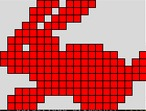
\includegraphics[width=0.25\textwidth]{rabbit.jpg}
    \caption{Example of a solved nonogram-puzzle. The red boxes marks cells
    that are common for both column and row.} 
    
\end{figure}

\noindent
\textbf{variables}: Consider the figure of the rabbit. The first row consists of the feet of the rabbit, where the feet touches the ground.
The segment lengths are 4 and 5. The variable here is defined as the entries in the row.
Therefore, we have a single variable for the first row, with the value $[0, 1, 1, 1, 1, 0, 0, 0, 0, 0, 0, 1, 1, 1, 1, 1, 0, 0, 0, 0]$.

In general, we have rows with dimensionality $M$ and columns with dimensionality $N$. Thus, a variable for a row is a vector
$x \in \{0, 1\}^M$ and for a column a vector $y \in \{0, 1\}^N$.\\

\noindent
\textbf{domains}: For each variable $x$ the domain $\mathcal{D}(x)$ is
defined as all feasible values for the variable.  Consider a column with length
$N$ and with $n$ segments, each with length $l_1,\ldots, l_n$. The total
length is $L = \sum_i^N l_i$. For the first segment, the first index the first
cell can be placed is 0.  The last index is found by $M - (n-1) - L$ because the
expression $L + (n-1)$ represent the minimum space occupied by all cells.
For example, we can see in the first row that $M = 20$, $L = 4 + 5 = 9$ and $n-1 = 1$.
From this we can deduce that the last index that the first segment can start on
is $20 - 9 - 1 = 10$. A recursive procedure is applied that finds the domains
for each variable\\

\noindent
\textbf{constraints}: The discussion above showed how the domains of each
variable is found. We can restrict the domain size by enforcing the domain
size for each row and column.  This will generate a list of possible rows for
each row and a list of possible columns for each column.

Furthermore, each column and row must agree with each other on which cells are marked
and which are not. Any row that marks a cell that is for certain not in the
corresponding column must be removed. Similarly, any column that marks a cell
that is for certain not in the corresponding row must be removed. Pseudocode
of this filtering algorithm is shown below.\\

% \begin{algorithm}
%     \begin{small}
%         \begin{lstlisting}[language=Python, caption=Generation of row / column segments]
% def generate_segments(seg_lengths, tot_length,
%                       min_idx=0,  index=0,
%                       segment=None):
% 
%   if index == 0:  # we're in the base case -- make an empty line
%     segment = np.zeros(tot_length, dtype=np.int64)
% 
%   n_remaining = len(seq_lengths[index:])
%   length_ahead = seg_lengths[index:].sum() + (n_remaining - 1)
% 
%   max_idx = tot_length - length_ahead
% 
%   # place current segment on all possible places
%   for i in range(min_idx, max_idx + 1):
%    new_segment = copy.deepcopy(segment)
%    new_segment[i:i + seg_lengths[index]] = np.int64(1)
%    min_idx_prime = i + seg_lengths[index] + 1
% 
%   is_last_index = index == len(seg_lengths) - 1
%    if is_last_index:  # finished
%      yield new_segment
% 
%    else:  # fix the segment and find remaining possible domains
%      for each in generate_segments(seg_lengths, tot_length,
%                                    min_idx_prime, index+1, new_segment):
%        yield each
% 
%         \end{lstlisting}
%     \end{small}
% \end{algorithm}
% 
% \begin{algorithm}
%     \begin{small}
%         \begin{lstlisting}[language=Python, caption=Filtering of rows (columns) based on entries in columns (rows)]
%         function filter_X_on_Y(X, Y):
%           for y in Y:
%             common_cells = find_common_cells(y)
%             X = remove_x_where_not_present(common_cells)
%           return X
%         \end{lstlisting}
%     \end{small}
% \end{algorithm}
% 
% ..
% 
